\chapter{検証実験}\label{chap:experiment}

\section{概要}
本論文で提案する個人認証システムについて,以下の3つの評価実験を行った.
\begin{description}
  \item[Manual Modeを用いた認証方式の評価実験] SNSの情報を利用することで,従来のPINを一桁増やした認証と比較し,どれだけ利便性と安全性を向上させることができるかを検証する
  \item[Auto Mode Type Termを用いた認証方式の評価実験] 一定のルール(期間)に基づいて秘密情報が変化することが認証の成功率やユーザへの負担にどう影響を与えるかについて検証する
  \item[Auto Mode Type Cycleを用いた認証方式の評価実験] 一定のルール(周期)に基づいて秘密情報が変化することが認証の成功率やユーザへの負担にどう影響を与えるかについて検証する
\end{description}
それぞれの実験は,時間的な制約から予備実験,本実験などの形式で行うことをせず,一度に行った.
また,ユーザからみた利便性に対する評価を得るするため,2回の選択式(一部自由記述含む)アンケートを実施した.

\subsection{実験手順}
以降の節のそれぞれの実験は第\ref{subsec:selectSecret}節にて挙げた3つの実装(以降,「パターン」と記載する)に対応しており,それぞれのパターンは多要素化手法として評価するために認証操作の後に4桁のPINによる認証操作を追加した.
そこに「PINの桁数を一桁増やし,5桁にしたものを秘密情報とする」パターンを追加し,計4パターンで相互に比較を行った.
各パターンの実験は一つにつき8日間にわたって実施,その間に設定した日から数えて,0日目(設定直後),1日目,3日目,8日目の4回の認証試行を行った(図\ref{fig:schedule}).
それぞれのパターンで実験中の期間は重複せず,順番は偏りのないように設定し,そのスケジュールにそって全実験を実施した.
また,アンケートに関しては,16日目が経過した段階で,2種類のパターンを比較するための中間アンケート(付録\ref{apdx:interimEnquete})を,32日目が経過した段階で最終アンケート(付録\ref{apdx:finalEnquete})を行った.
\footnote{スケジュールは4つのパターンの組み合わせであり,その総数は$ {}_4 P _4 $の式で表される.
本実験ではこれら全てに固有の番号(以降,「スケジュール番号」と記載する)を付録\ref{apdx:schedule}の通り割り振って管理する.}

\begin{figure}[ht]
  \begin{center}
    \epsfig{file=img/schedule.pdf,scale=1.1}
  \end{center}
  \caption{実験スケジュール}
  \label{fig:schedule}
\end{figure}

\subsubsection{初回実験説明・導入}
\begin{enumerate}
  \item 実験担当者が実験の目的・注意事項・免責事項を説明する.この手順は付録\ref{apdx:experiment}の実験説明資料と操作説明資料を用いて行い,不明な点があれば質問してもらった.
  \item 被験者のスケジュールを決定し,それに合わせて提案システムを実装したアプリケーションソフトウェア(以降「Notifauth」と記載する)のソースコードにスケジュール番号を登録した.
  \item 実験担当者の開発用端末と被験者の携帯端末を接続し,Notifauthをインストールする\footnote{ここでAppleの開発者用アカウントと被験者の端末の紐付けを行う}.
  \item 実際にNotifauthを操作し,全てのパターンでひと通りの秘密情報設定と認証操作を行ってもらった.
  \item その後,Notifauth内の全ての保存されたデータを初期化し,スケジュールに沿ったパターンのみ設定を行ってもらうことで実験開始とした.
  \item 上記手順で設定したパターンについて認証操作を行ってもらった.
  \item この段階で実験データを送信してもらい,該当データの受信を実験担当者が確認を行った.
\end{enumerate}

\subsubsection{試行手順}
\begin{enumerate}
  \item トップ画面(付録\ref{apdx:screen}内の図\ref{fig:notifauthHome})で,試行したいパターンをセレクタで選択し,「Test」をタップする.
  \item ``PIN Mode''以外の場合,ロック画面を模した画面(第\ref{sec:authentication}内の図\ref{fig:notifauthTest}左図)が表示され,秘密情報に当てはまると思われるツイートを見つけ,そのセルをスライドする.
  \item PINの入力画面(第\ref{sec:authentication}内の図\ref{fig:notifauthTest}右図)が表示され,``PIN Mode''であれば5桁,それ以外のパターンであれば4桁のPINを入力する.
  \item 結果画面が表示されるので,「Home」ボタンを押する.
\end{enumerate}

なお,試行手順の一つとして、実験結果は認証操作直後にメールで送信して頂くかたちで収集した.

\subsection{被験者}
男性12名,女性3名の計15名が実験を行った.
うち本学の学生は5名であった.
性別や年齢は表\ref{fig:participants}の通りである.
実験の開始時期の関係から,全員が実験を完了しているわけではなく,全ての検証実験を終了したのは10人で,そのうち最終アンケートに答えたのは7人である.
中間アンケートには12人が回答した.

\begin{figure}[ht]
  \begin{minipage}{0.32\hsize}
    \begin{center}
      \includegraphics[width=50mm]{resource/users_gender.pdf}
    \end{center}
  \end{minipage}
  \begin{minipage}{0.32\hsize}
    \begin{center}
      \includegraphics[width=50mm]{resource/users_age.pdf}
    \end{center}
  \end{minipage}
  \begin{minipage}{0.32\hsize}
    \begin{center}
      \includegraphics[width=50mm]{resource/users_tweet.pdf}
    \end{center}
  \end{minipage}
  \caption{被験者の特性(左:性別,中央:年齢,右:1日あたりのツイート数)}
  \label{fig:participants}
\end{figure}

%\begin{table}[ht]
%  \caption{被験者の特性}
%  \label{tab:participants}
%  \begin{minipage}{0.25\hsize}
%    \begin{center}
%      \small
%      \begin{tabular}{lr}
%        \bhline
%        \multicolumn{2}{l}{性別} \\ \hline
%        男性 & 15 \\
%        女性 & 3 \\
%        \bhline
%      \end{tabular}
%    \end{center}
%  \end{minipage}
%  \begin{minipage}{0.25\hsize}
%    \begin{center}
%      \small
%      \begin{tabular}{lr}
%        \bhline
%        \multicolumn{2}{l}{年齢} \\ \hline
%        10代 & 0 \\
%        20代 & 12 \\
%        30代 & 2 \\
%        40代 & 1 \\
%        50代以上 & 0 \\
%        \bhline
%      \end{tabular}
%    \end{center}
%  \end{minipage}
%  \begin{minipage}{0.25\hsize}
%    \begin{center}
%      \small
%      \begin{tabular}{lr}
%        \bhline
%        \multicolumn{2}{l}{1日の平均ツイート数} \\ \hline
%        0-1 & 0 \\
%        2-10 & 0 \\
%        11-50 & 0 \\
%        50-100 & 0 \\
%        100- & 0 \\
%        \bhline
%      \end{tabular}
%    \end{center}
%  \end{minipage}
%\end{table}

\section{Manual Modeを用いた認証方式の評価実験}\label{sec:vsTweet}
\subsection{概要}
本実験では,SNSの情報を利用することで,従来のPINを一桁増やした認証と比較し,どれだけ利便性と安全性を向上させることができるかの評価を行う.
本実験で評価対象とするパターンとして,``Manual Mode''を採用する.

\subsection{目的}
アプリケーションを用いた実験では,測定した結果から以下の3指標にもとづいて相関や有意差をみた.
\begin{itemize}
  \item 短期の記憶保持
    \begin{description}
      \item[目的] 秘密情報の短期記憶が可能かどうかの検証
      \item[仮説] 日数をおかない試行において5桁のPIN認証よりも認証成功率が高い,つまり,短期の記憶保持について暗証番号認証よりも当方式を用いた認証の方が容易
      \item[測定方法] 0日目,1日目,3日目の認証成功率を比較し,相関をみる
    \end{description}
  \item 長期の記憶保持
    \begin{description}
      \item[目的] 秘密情報の長期記憶が可能かどうかの検証
      \item[仮説] 日数をおく試行において5桁のPIN認証よりも認証成功率が高い,つまり,長期の記憶保持について暗証番号認証よりも当方式を用いた認証の方が容易
      \item[測定方法] 3日目と8日目の認証成功率を比較し,相関をみる.
    \end{description}
  \item 認証時間
    \begin{description}
      \item[目的] 利便性の検証
      \item[仮説] 5桁のPIN認証よりも認証時間が短い,つまり,暗証番号認証よりも当方式を用いた認証の方が利便性が高い
      \item[測定方法] 認証操作の画面が表示されてから,認証を終えるまでの時間を計測する.認証の成否は問わないものとする.
    \end{description}
\end{itemize}

\subsection{方法}
被験者実験により各試行の成功と失敗,認証にかかった時間を収集し,事後アンケートを実施する.
また,有意差はWelchのt検定を用いる(この場合,(1)サンプルサイズが30以上で十分大きいこと,(2)検定を複数回繰り返すことで帰無仮説全体を通しての有意水準が不当に上昇してしまう,(3)t検定は母分布が正規分布でないときにも頑健性を持つ(妥当な結果を与える),ことから,標本が正規分布であることは検証をせずに自明とした.

\subsection{結果}
本実験の結果を表\ref{tab:manual.data}に示す.
試行のタイミングが1日程度前後した被験者が存在したため,1-2日目を1日目,3-6日目におこなったものを3日目,7-8日目に行ったものを8日目の試行とした.
比較のためのPIN Modeにおける認証成功率と認証時間は表\ref{tab:manual.data}に示す.

\begin{table}[t]
  \caption{Manual Modeにおける各経過日数ごとの認証成功率と認証時間の変化($ n = 51 $)}
  \label{tab:manual.data}
  \begin{center}
    \small
    \begin{tabular}{rrr}
      \bhline
      経過日数 & 認証成功率(\%) & 認証時間(秒)\\ \hline
      0    & 92.9 & 14.2 \\
      1-2 & 91.7 & 10.7 \\
      3-6 & 91.7 & 8.9 \\
      7-8 & 100.0 & 8.7 \\ \hline \hline
      平均 & 94.12 & 10.74 \\
      標準偏差 & 3.47 & 8.61 \\
      中央値       & & 7.86 \\
      最大値       & & 41.84 \\
      最小値       & & 3.29 \\
      \bhline
    \end{tabular}
  \end{center}
\end{table}

\begin{table}[b]
  \caption{PIN Modeにおける各経過日数ごとの認証成功率と認証時間の変化($ n = 51 $)}
  \label{tab:manual.data}
  \begin{center}
    \small
    \begin{tabular}{rrr}
      \bhline
      経過日数 & 認証成功率(\%) & 認証時間(秒)\\ \hline
      0    & 100.0 & 2.17 \\
      1-2 & 92.3 & 2.81 \\
      3-6 & 90.9 & 2.82 \\
      7-8 & 100.0 & 2.51 \\ \hline \hline
      平均 & 96.08 & 2.55 \\
      標準偏差 & 4.22 & 1.60 \\
      中央値       & & 1.93 \\
      最大値       & & 8.40 \\
      最小値       & & 1.11 \\
      \bhline
    \end{tabular}
  \end{center}
\end{table}

\begin{figure}[t]
  \begin{center}
    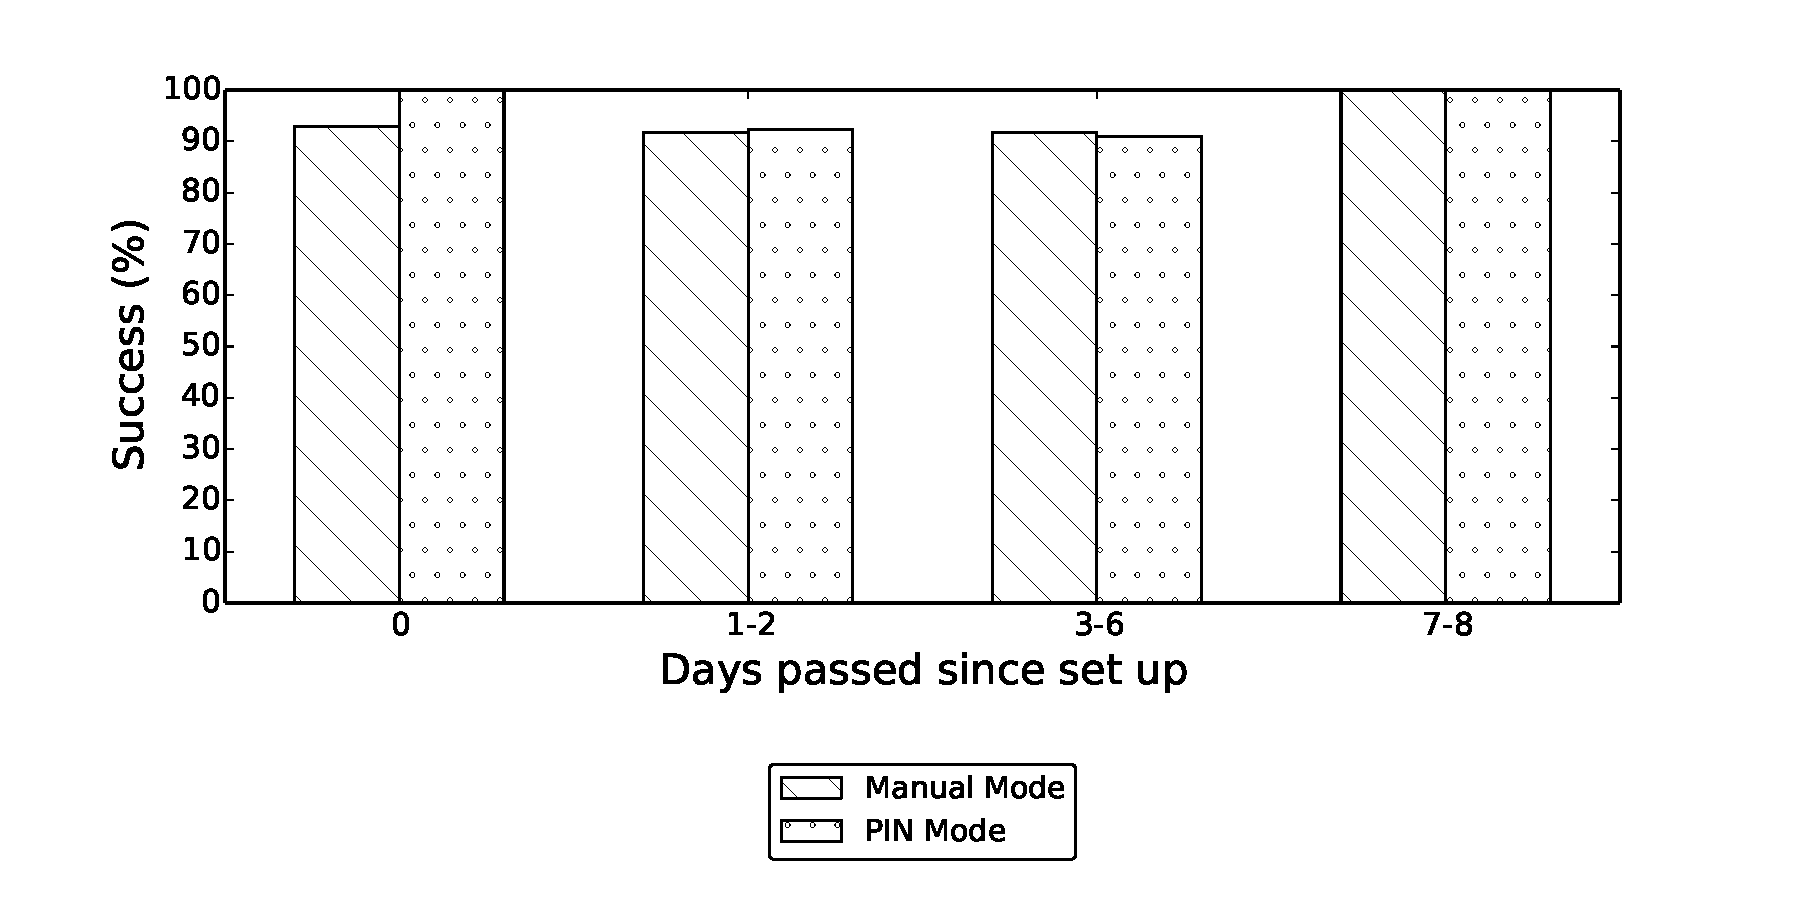
\epsfig{file=resource/ex_manual_vs_pin_rate.pdf,scale=0.5}
  \end{center}
  \caption{Manual ModeとPIN Modeにおける設定時からの経過日数ごとの認証成功率}
  \label{fig:ex_manual_vs_pin_rate}
\end{figure}

\begin{figure}[b]
  \begin{center}
    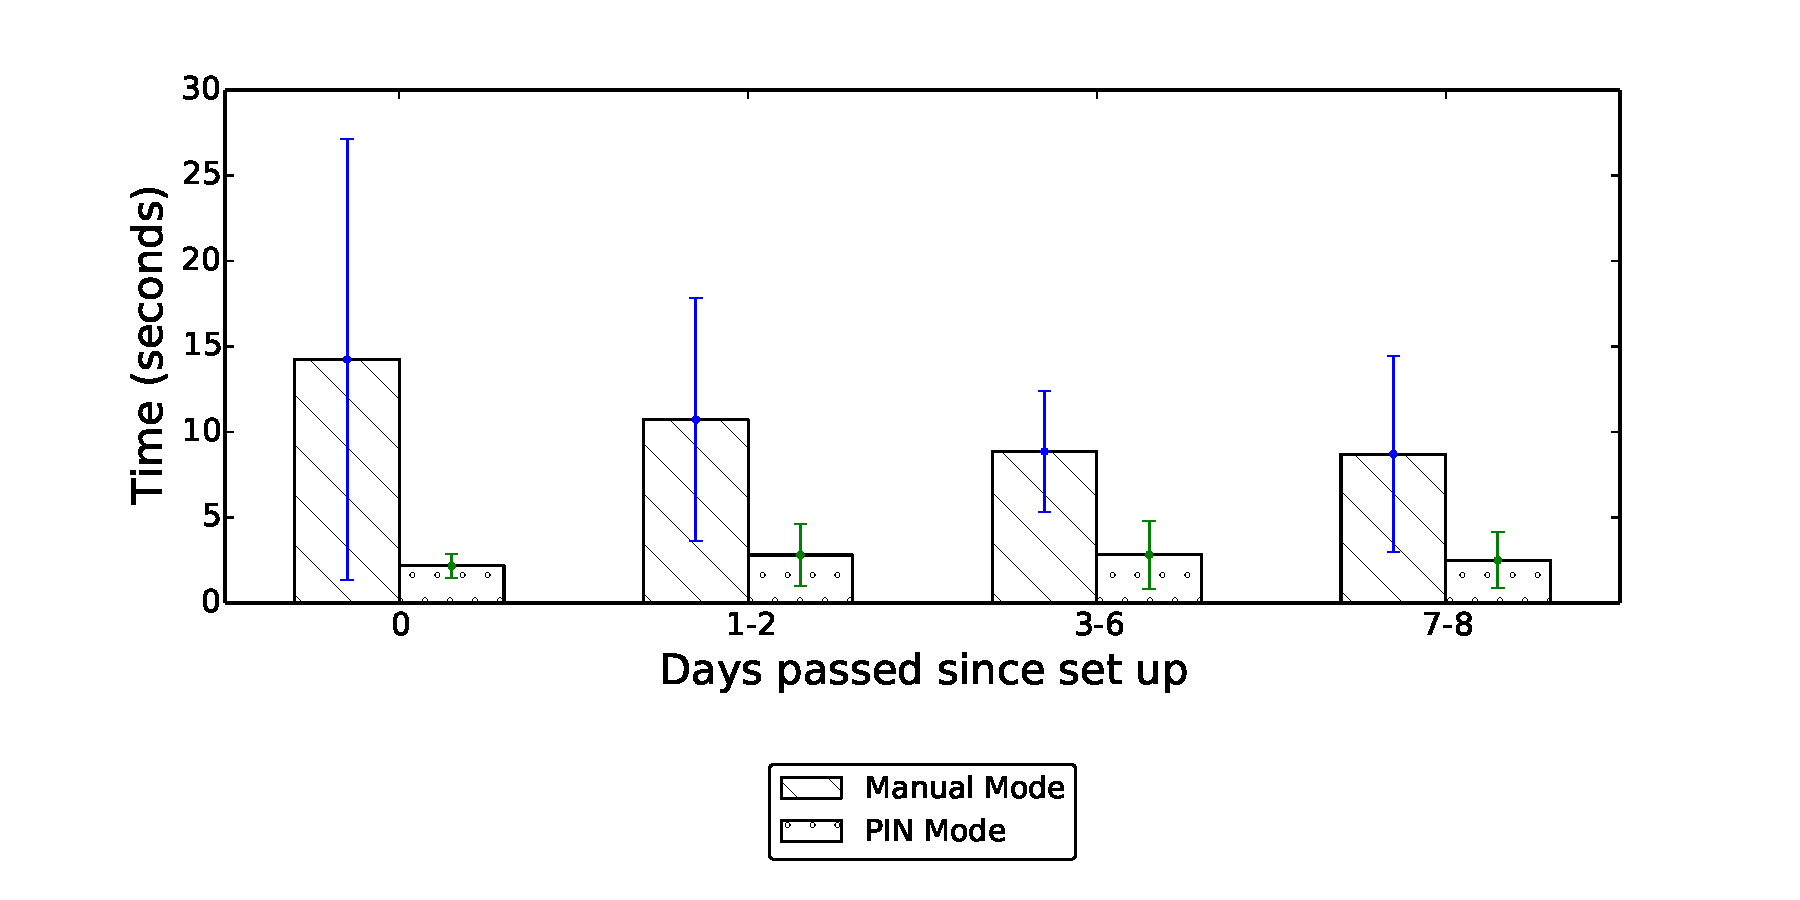
\epsfig{file=resource/ex_manual_vs_pin_time.pdf,scale=0.5}
  \end{center}
  \caption{Manual ModeとPIN Modeにおける設定時からの経過日数ごとの認証時間}
  \label{fig:ex_manual_vs_pin_time}
\end{figure}

\subsubsection{記憶保持}
表\ref{tab:manual.data}に示した通り,経過日数と認証成功率におけるピアソンの相関係数は0.144で,標本数による限界値\cite{978-4641121607}を考慮しても有意な差ではないと考えられる.
また,図\ref{fig:ex_manual_vs_pin_rate}にPIN Modeとの認証率の比較を示した.
検定を行った結果,PIN Modeの認証成功率とは有意差がある(Welchのt検定,$ p = 0.012 < 0.05 $)ことが明らかになった.

\begin{itemize}
  \item 短期の記憶保持
\end{itemize}
0日目,1日目,3日目にかけてのManual Modeでの認証成功率は92.9\%,91.7\%,91.7\%と推移しており,ピアソン相関係数は0.031で,有意な相関はみられなかった.

\begin{itemize}
  \item 長期の記憶保持
\end{itemize}
3日目の認証成功率は91.7\%で,8日目には100\%であった.
3日目から8日目にかけてのピアソン相関係数は0.261であり,有意な相関はみられなかった.

\subsubsection{認証時間}
図\ref{fig:ex_manual_vs_pin_time}にManual ModeとPIN Modeとの認証時間の比較を示した.
PIN Modeとは数値上4倍程度の差があり,検定を行った結果,有意差がある(Welchのt検定,$ p = 0 $)といえた.

\subsubsection{アンケート結果}
表\ref{tab:auto_term.enquete}に被験者によるアンケート結果を示す.
また,PIN Modeに対するアンケート結果も併せて表\ref{tab:pin.enquete}に示す.

\begin{table}[t]
  \caption{被験者によるManual Modeに対するアンケート内評価}
  \label{tab:manual.enquete}
  \begin{center}
    \small
    \begin{tabular}{lrr}
      \bhline
      項目名 & 平均値 & 回答者数 \\ \hline
      秘密情報の記憶保持にかかわる負担はどのくらい感じますか? & 1.13 & 8 \\
      (とても小さい:1-とても大きい:5) & & \\
      認証にかかる時間はどのように感じましたか? & 1.13 & 8 \\
      (とても短い:1-とても長い:5) & & \\
      認証を成功させるために必要な操作負担はどの程度でしたか? & 1.25 & 8 \\
      (とても小さい:1-とても大きい:5) & & \\
      認証を行うのにどれくらいフラストレーションを感じましたか? & 1.5 & 8 \\
      (とても小さい:1-とても大きい:5) & & \\
      タイピングしたりタッチパネルをスライドしたりする作業の & 1.43 & 7 \\
      負担はどの程度でしたか?(とても小さい:1-とても大きい:5) & & \\
      \bhline
    \end{tabular}
  \end{center}
\end{table}
\begin{table}[b]
  \caption{被験者によるPIN Modeに対するアンケート内評価}
  \label{tab:pin.enquete}
  \begin{center}
    \small
    \begin{tabular}{lrr}
      \bhline
      項目名 & 平均値 & 回答者数 \\ \hline
      秘密情報の記憶保持にかかわる負担はどのくらい感じますか? & 1.13 & 8 \\
      (とても小さい:1-とても大きい:5) & & \\
      認証にかかる時間はどのように感じましたか? & 1.13 & 8 \\
      (とても短い:1-とても長い:5) & & \\
      認証を成功させるために必要な操作負担はどの程度でしたか? & 1.13 & 8 \\
      (とても小さい:1-とても大きい:5) & & \\
      認証を行うのにどれくらいフラストレーションを感じましたか? & 1.5 & 8 \\
      (とても小さい:1-とても大きい:5) & & \\
      タイピングしたりタッチパネルをスライドしたりする作業の & 1.43 & 7 \\
      負担はどの程度でしたか?(とても小さい:1-とても大きい:5) & & \\
      \bhline
    \end{tabular}
  \end{center}
\end{table}

\section{Auto Mode Type Termを用いた認証方式の評価実験}\label{sec:vsTerm}
\subsection{概要}
本実験では,SNSの情報の特性を利用した認証システムとして``Auto Mode Type Term''を採用し,記憶持続性と利便性の評価を行う.
更に,ある一定のルールに基づいて秘密情報が変化することが認証の成功率やユーザへの負担がどう影響を与えるかについても検証する.
また,他の実験で用いたパターンとの比較も行う.

\subsection{目的}
アプリケーションを用いた実験で測定した結果から相関や有意差をみた指標は第\ref{sec:vsTweet}節に準じ,(1)短期の記憶保持,(2)長期の記憶保持,(3)認証時間とした.

\subsection{方法}
被験者実験により各試行の成功と失敗,認証にかかった時間を収集し,事後アンケートを実施する.
平均値を比較する際の検定方法は\ref{sec:vsTweet}節に準じ,Welchのt検定を利用した.

\subsection{結果}
本実験の結果を表\ref{tab:auto_term.data}に示す.
試行のタイミングが1日程度前後した被験者が存在したため,1-2日目を1日目,3-6日目におこなったものを3日目,7-8日目に行ったものを8日目の試行とした.
比較のためのPIN Modeにおける認証成功率と認証時間は第\ref{sec:vsManual}節と同じく表\ref{tab:manual.data}に示す.
\begin{table}[ht]
  \caption{Auto Mode Type Termにおける各経過日数ごとの認証成功率と認証時間の変化($ n = 58 $)}
  \label{tab:auto_term.data}
  \begin{center}
    \small
    \begin{tabular}{rrr}
      \bhline
      経過日数 & 認証成功率(\%) & 認証時間\\ \hline
      0   & 40.0 & 21.52 \\
      1-2 & 38.5 & 21.67 \\
      3-6 & 75.0 & 20.30 \\
      7-8 & 41.7 & 19.09 \\ \hline \hline
      平均 & 51.79 & 22.14 \\
      標準偏差 & 14.39 & 14.50 \\
      中央値     & & 19.24 \\
      最大値     & & 65.0 \\
      最小値     & & 5.62 \\
      \bhline
    \end{tabular}
  \end{center}
\end{table}

\begin{figure}[ht]
  \begin{center}
    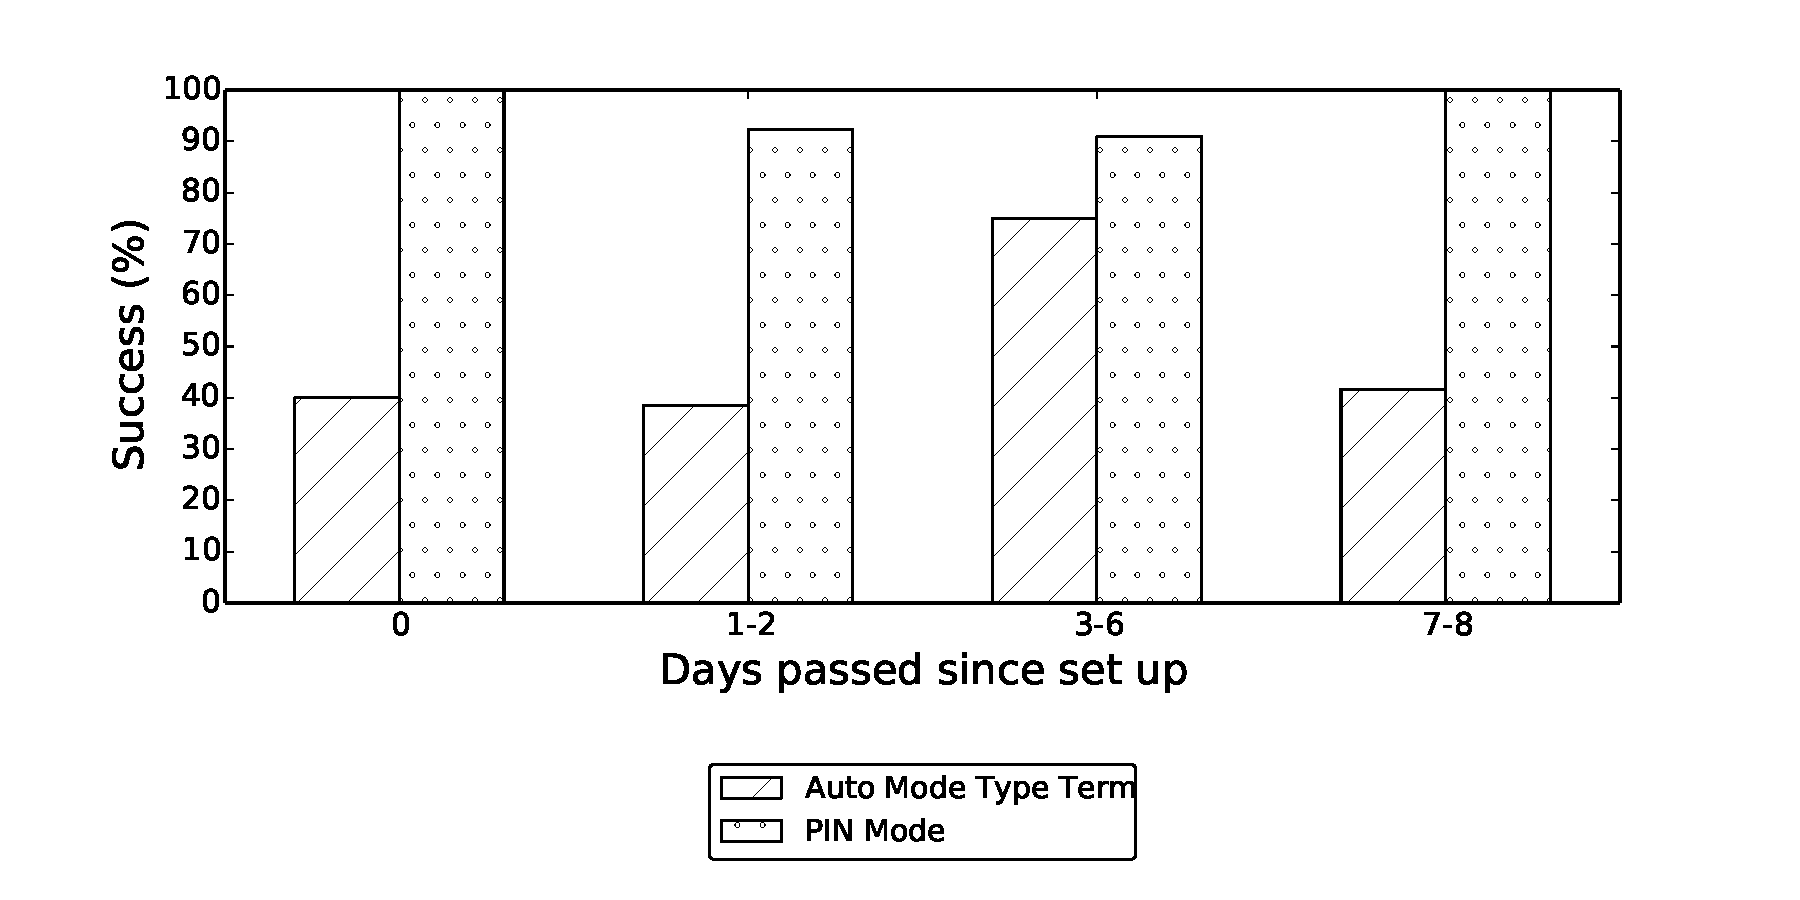
\epsfig{file=resource/ex_auto_term_vs_pin_rate.pdf,scale=0.5}
  \end{center}
  \caption{Auto Mode Type TermとPIN Modeにおける設定時からの経過日数ごとの認証成功率}
  \label{fig:ex_auto_term_vs_pin_rate}
\end{figure}

\begin{figure}[hb]
  \begin{center}
    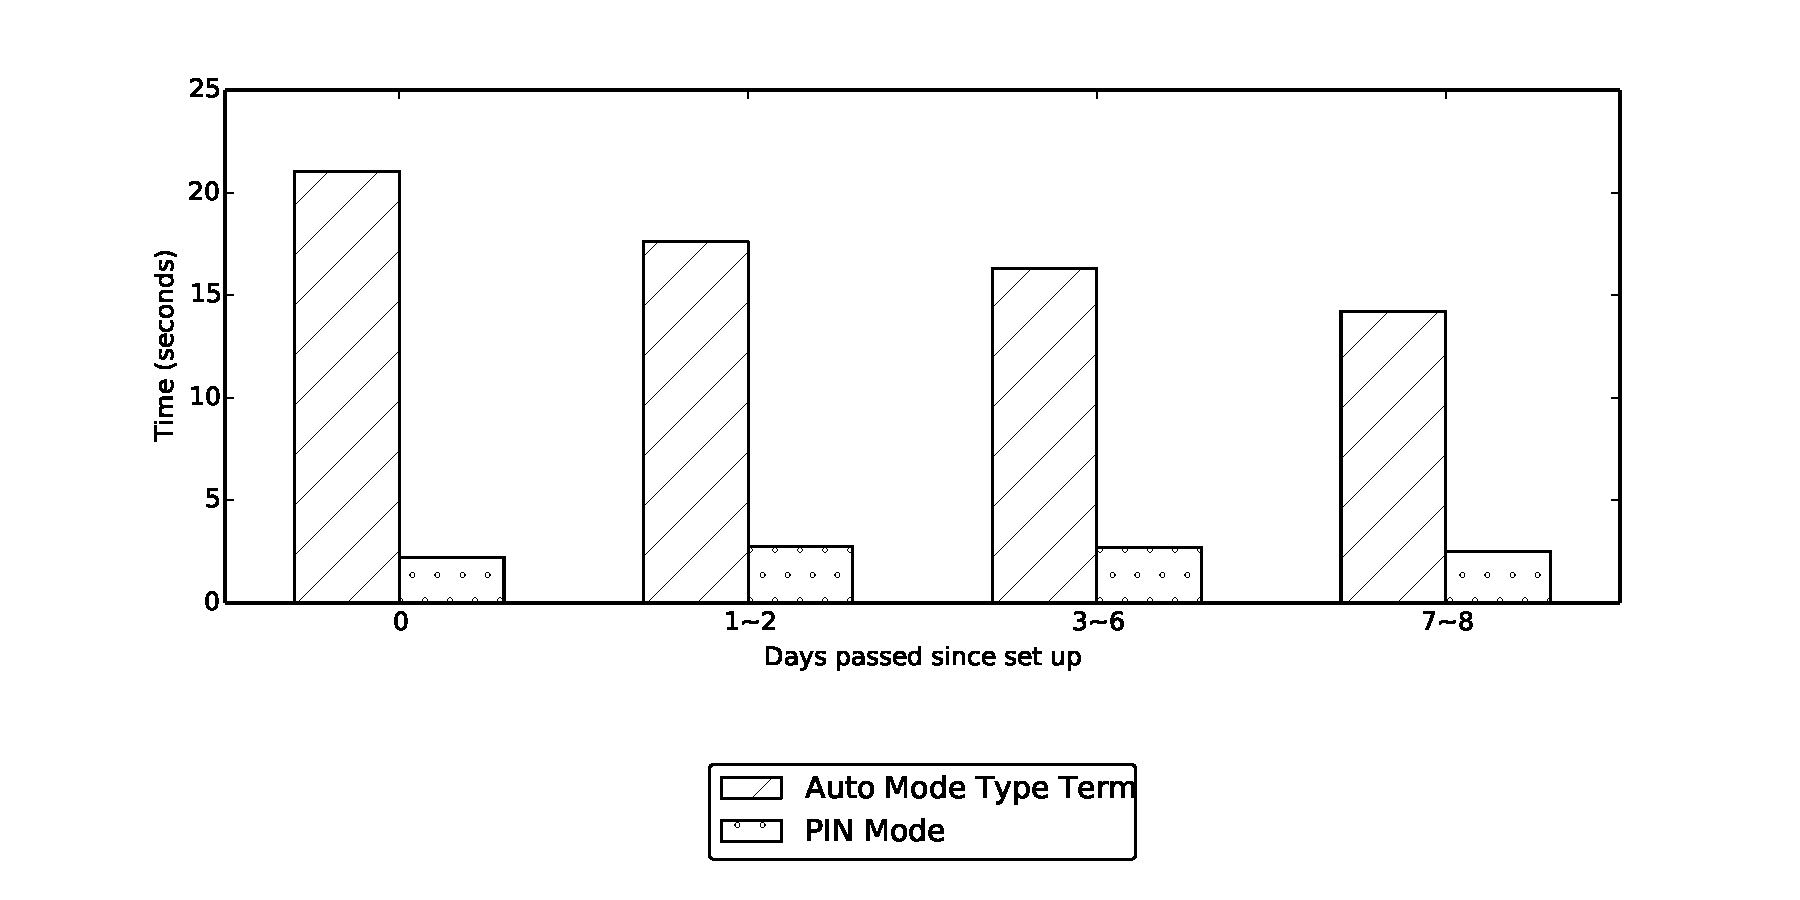
\epsfig{file=resource/ex_auto_term_vs_pin_time.pdf,scale=0.5}
  \end{center}
  \caption{Auto Mode Type TermとPIN Modeにおける設定時からの経過日数ごとの認証時間}
  \label{fig:ex_auto_term_vs_pin_time}
\end{figure}

\subsubsection{記憶保持}
表\ref{tab:auto_term.data}に示した通り,経過日数と認証成功率におけるピアソンの相関係数は0.234で,標本数による限界値を考慮すると有意ではないと考えられる.
また,図\ref{fig:ex_auto_term_vs_pin_rate}にPIN Modeとの認証率の比較を示した.
検定を行った結果,PIN Modeの認証成功率とは有意差がある(Welchのt検定,$ p = 0 $)ことが明らかになった.
\begin{itemize}
  \item 短期の記憶保持
\end{itemize}
0日目から3日目までのManual Modeでの認証成功率は38.5\%から75.0\%とばらつきがみられ,ピアソン相関係数は0.233で有意な相関ではない.

\begin{itemize}
  \item 長期の記憶保持
\end{itemize}
3日目の認証成功率は75.0\%,8日目の認証成功率は41.7\%で,期間が空くと認証成功率が下がってしまった.
3日目から8日目の期間におけるピアソン相関係数は-0.347で,相関はみられなかった.

\subsubsection{認証時間}
図\ref{fig:ex_auto_term_vs_pin_time}にPIN Modeとの認証時間の比較を示した.
こちらもManual Mode同様,PIN Modeとは大きく差があり,検定を行った結果,有意差がある(Welchのt検定,$ p = 0 $)ことが判明した.

\subsubsection{アンケート結果}
被験者によるアンケート結果を表\ref{tab:auto_term.enquete}に記す.
この認証方法で失敗したことがあると答えた人の中で,設定内容を覚えていた人は7人中4人で,設定内容を忘れてしまった人は7人中3人であった.

\begin{table}[ht]
  \caption{被験者によるAuto Mode Type Termに対するアンケート内評価}
  \label{tab:auto_term.enquete}
  \begin{center}
    \small
    \begin{tabular}{lrr}
      \bhline
      項目名 & 平均値 & 回答者数 \\ \hline
      秘密情報の記憶保持にかかわる負担はどのくらい感じますか? & 4.09 & 11 \\
      (とても小さい:1-とても大きい:5) & & \\
      認証にかかる時間はどのように感じましたか? & 3.73 & 11 \\
      (とても短い:1-とても長い:5) & & \\
      認証を成功させるために必要な操作負担はどの程度でしたか? & 3.18 & 11 \\
      (とても小さい:1-とても大きい:5) & & \\
      認証を行うのにどれくらいフラストレーションを感じましたか? & 3.45 & 11 \\
      (とても小さい:1-とても大きい:5) & & \\
      タイピングしたりタッチパネルをスライドしたりする作業の & 3.14 & 7 \\
      負担はどの程度でしたか?(とても小さい:1-とても大きい:5) & & \\
      \bhline
    \end{tabular}
  \end{center}
\end{table}

\section{Auto Mode Type Cycleを用いた認証方式の評価実験}\label{sec:vsCycle}
\subsection{概要}
本実験では,SNSの情報の特性を利用した認証システムとして``Auto Mode Type Cycle''を採用し,記憶持続性と利便性の評価を行う.
更に,ある一定のルールに基づいて秘密情報が変化することが認証の成功率やユーザへの負担がどう影響を与えるかについても検証する.
また,他の実験で用いたパターンとの比較も行う.

\subsection{目的}
アプリケーションを用いた実験で測定した結果から相関や有意差をみた指標は第\ref{sec:vsTweet}節に準じ,(1)短期の記憶保持,(2)長期の記憶保持,(3)認証時間とした.

\subsection{方法}
被験者実験により各試行の成功と失敗,認証にかかった時間を収集し,事後アンケートを実施する.
平均値を比較する際の検定方法は\ref{sec:vsTweet}節に準じ,Welchのt検定を利用した.

\subsection{結果}
本実験の結果を表\ref{tab:auto_cycle.data}に示す.
試行のタイミングが1日程度前後した被験者が存在したため,1-2日目を1日目,3-6日目におこなったものを3日目,7-8日目に行ったものを8日目の試行とした.
比較のためのPIN Modeにおける認証成功率と認証時間は第\ref{sec:vsManual}節と同じく表\ref{tab:manual.data}に示す.
\begin{table}[ht]
  \caption{Auto Mode Type Cycleにおける各経過日数ごとの認証成功率と認証時間の変化($ n = 58 $)}
  \label{tab:auto_cycle.data}
  \begin{center}
    \small
    \begin{tabular}{rrr}
      \bhline
      経過日数 & 認証成功率(\%) & 認証時間\\ \hline
      0   & 35.7 & 21.7 \\
      1-2 & 25.0 & 21.5 \\
      3-6 & 14.3 & 26.2 \\
      7-8 & 30.8 & 22.9 \\ \hline \hline
      平均 & 27.59 & 22.95 \\
      標準偏差 & 7.98 & 15.27 \\
      中央値   & & 20.1 \\
      最大値   & & 91.0 \\
      最小値   & & 4.99 \\
      \bhline
    \end{tabular}
  \end{center}
\end{table}

\begin{figure}[t]
  \begin{center}
    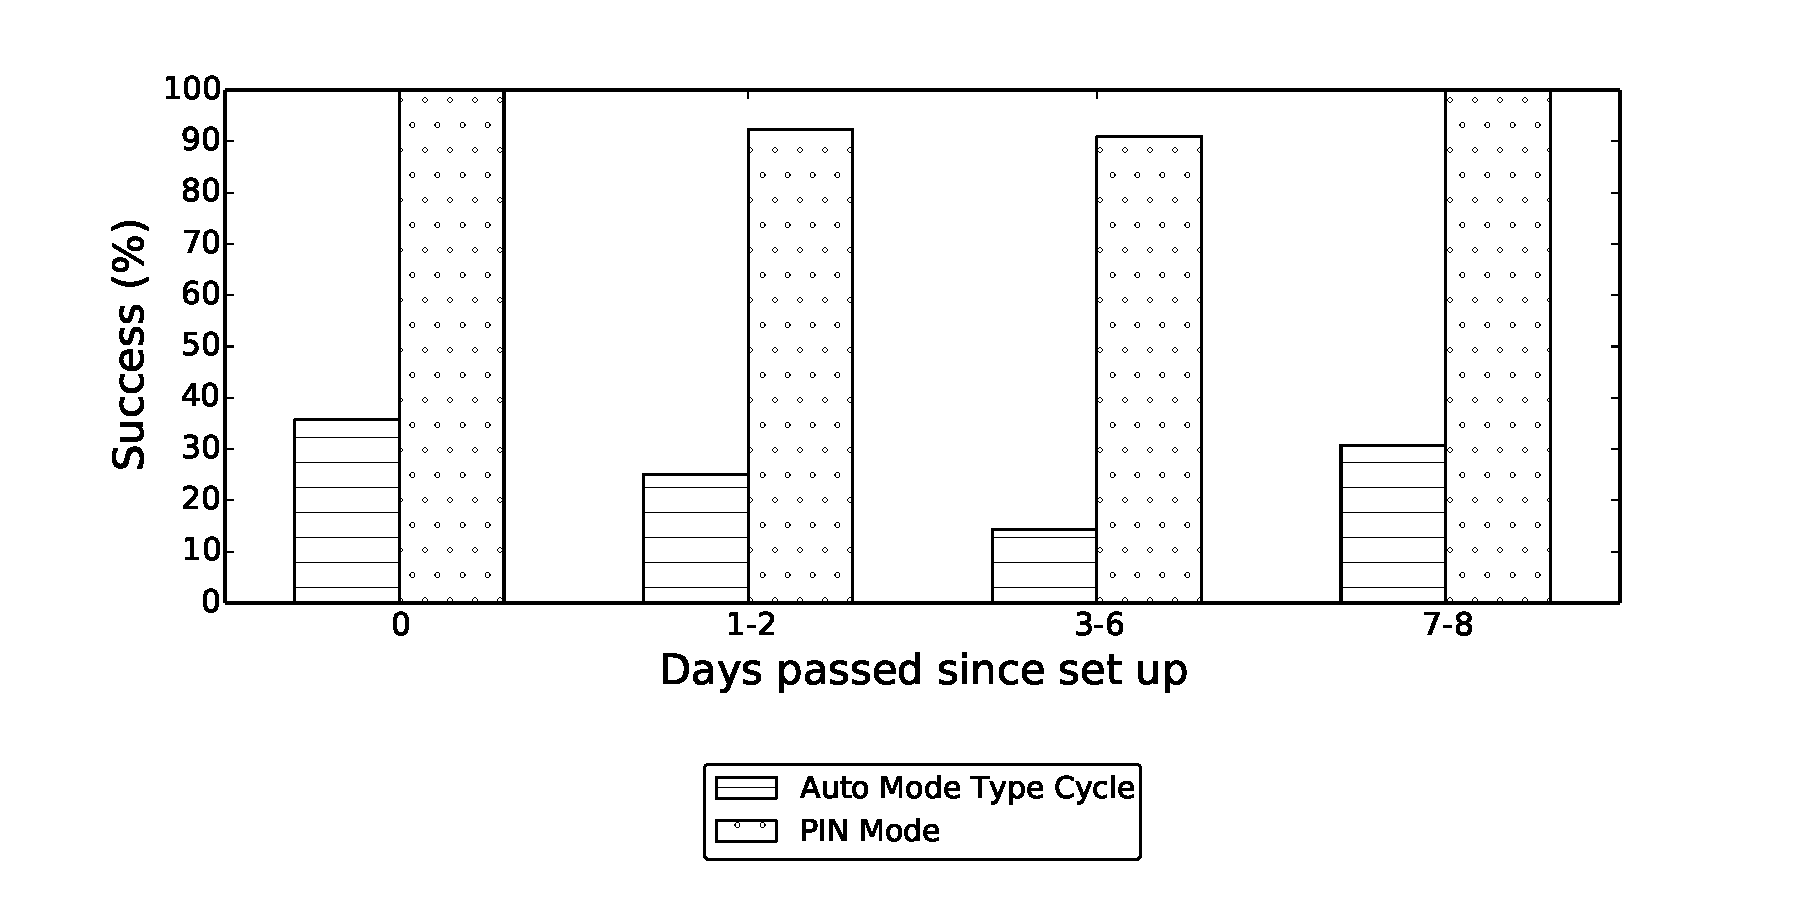
\epsfig{file=resource/ex_auto_cycle_vs_pin_rate.pdf,scale=0.5}
  \end{center}
  \caption{Auto Mode Type CycleとPIN Modeにおける設定時からの経過日数ごとの認証成功率}
  \label{fig:ex_auto_cycle_vs_pin_rate}
\end{figure}

\begin{figure}[b]
  \begin{center}
    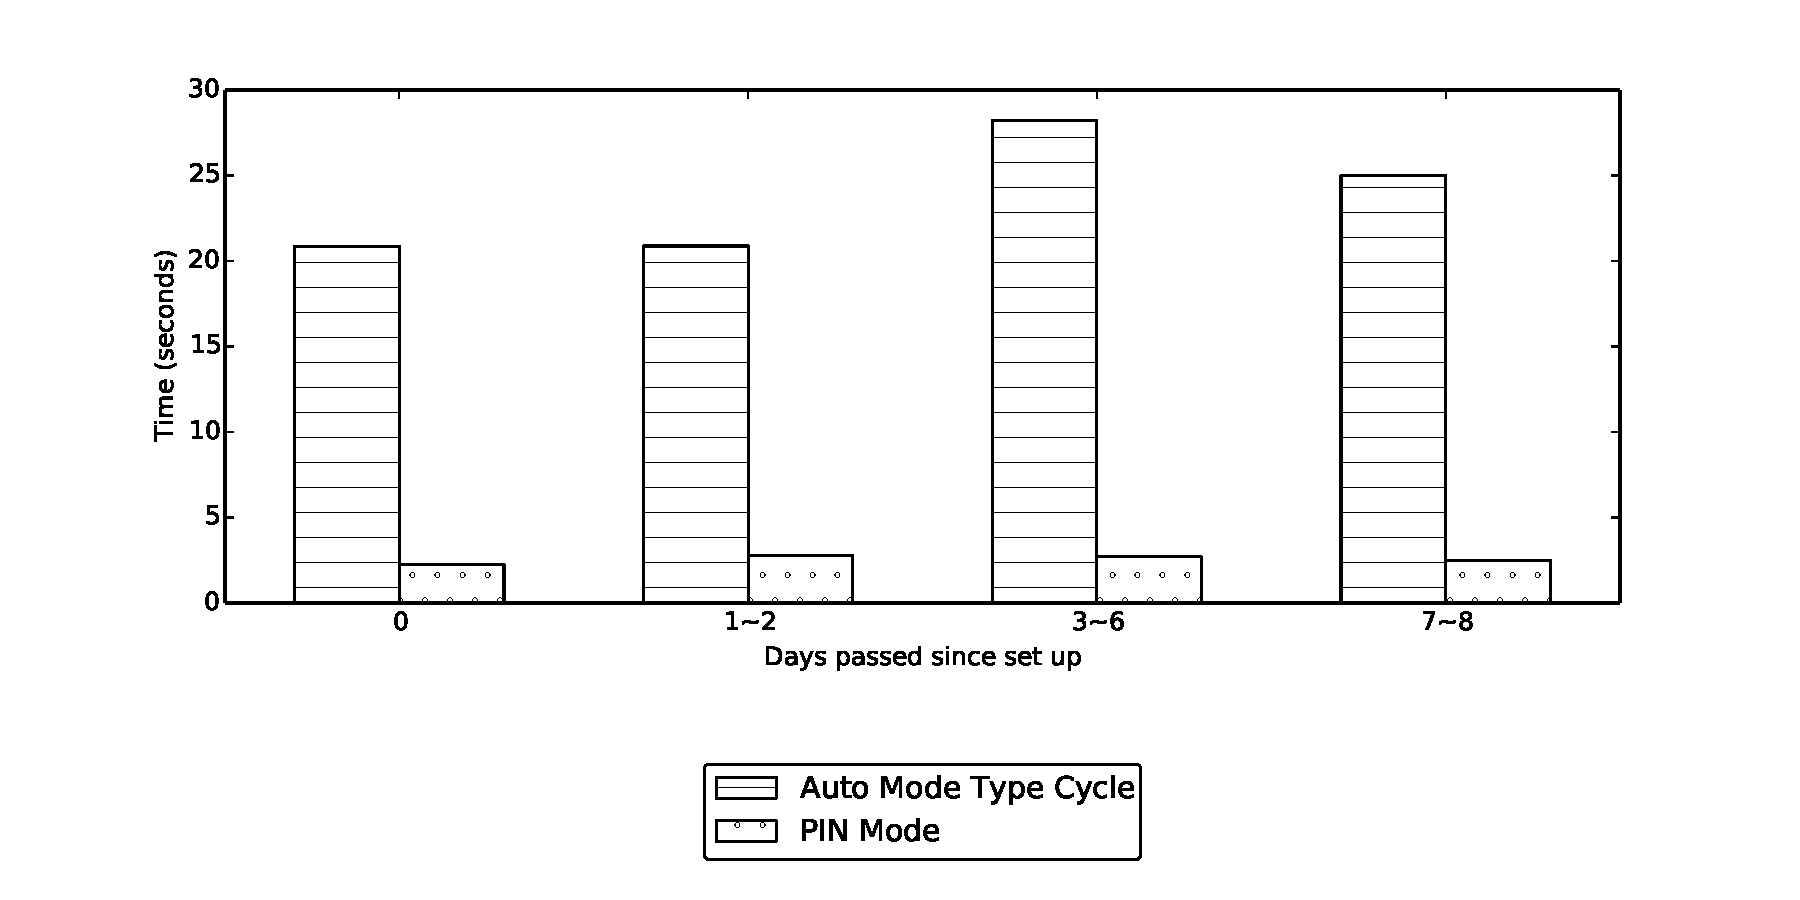
\epsfig{file=resource/ex_auto_cycle_vs_pin_time.pdf,scale=0.5}
  \end{center}
  \caption{Auto Mode Type CycleとPIN Modeにおける設定時からの経過日数ごとの認証時間}
  \label{fig:ex_auto_cycle_vs_pin_time}
\end{figure}

\subsubsection{記憶保持}
表\ref{tab:auto_cycle.data}に示した通り,経過日数と認証成功率におけるピアソンの相関係数は0.083で,標本数による限界値を考慮すると有意ではないと考えられる.
また,図\ref{fig:ex_auto_cycle_vs_pin_rate}にPIN Modeとの認証率の比較を示した.
検定を行った結果,PIN Modeの認証成功率とは有意差がある(Welchのt検定,$ p = 0 $)ことが明らかになった.
\begin{itemize}
  \item 短期の記憶保持
\end{itemize}
0日目から3日目までのAuto Mode Type Cycleにおける認証成功率は35.7\%から14.3\%まで落ちた.
この期間でのピアソン相関係数は-0.149であり,有意な相関はみられなかった.

\begin{itemize}
  \item 長期の記憶保持
\end{itemize}
3日目の認証成功率は14.3\%,8日目の認証成功率は30.8\%であり,ピアソン相関係数0.243と有意な相関はみられなかった.

\subsubsection{認証時間}
図\ref{fig:ex_auto_cycle_vs_pin_time}にPIN Modeとの認証時間の比較を示した.
こちらも他のMode同様,PIN Modeとは大きく差があり,検定を行った結果,有意差がある(Welchのt検定,$ p = 0 $)ことが判明した.

\subsubsection{アンケート結果}
被験者によるアンケート結果を表\ref{tab:auto_cycle.enquete}に記す.
この認証方法で失敗したことがあると答えた人の中で,設定内容を覚えていた人は7人中5人で,設定内容を忘れてしまった人は7人中2人であった.

\begin{table}[ht]
  \caption{被験者によるAuto Mode Type Cycleに対するアンケート内評価}
  \label{tab:auto_cycle.enquete}
  \begin{center}
    \small
    \begin{tabular}{lrr}
      \bhline
      項目名 & 平均値 & 回答者数 \\ \hline
      秘密情報の記憶保持にかかわる負担はどのくらい感じますか? & 3.56 & 11 \\
      (とても小さい:1-とても大きい:5) & & \\
      認証にかかる時間はどのように感じましたか? & 3.44 & 11 \\
      (とても短い:1-とても長い:5) & & \\
      認証を成功させるために必要な操作負担はどの程度でしたか? & 2.44 & 11 \\
      (とても小さい:1-とても大きい:5) & & \\
      認証を行うのにどれくらいフラストレーションを感じましたか? & 3.44 & 11 \\
      (とても小さい:1-とても大きい:5) & & \\
      タイピングしたりタッチパネルをスライドしたりする作業の & 2.57 & 7 \\
      負担はどの程度でしたか?(とても小さい:1-とても大きい:5) & & \\
      \bhline
    \end{tabular}
  \end{center}
\end{table}

%\section{各評価実験間での相互比較}\label{sec:vsAll}
%\subsection{目的}
%本節では,各評価実験で行ったパターン全てのなかで比較を行う.%

%\subsection{方法}
%被験者実験により各試行の成功と失敗,認証にかかった時間を収集する.
%また,付録の\ref{apdx:interimEnquete}や\ref{apdx:finalEnquete}にある通り,被験者には使用パターンについて5段階のリッカート尺度を使った質問に答えてもらい,さらに既に8日間の試行が終了している他パターンとの比較もしてもらう.%

%\subsection{結果}
%\subsubsection{期間と周期での比較}
%図\ref{fig:ex_auto_term_vs_auto_cycle_rate}と図\ref{fig:ex_auto_term_vs_auto_cycle_time}にAuto Modeの2タイプにおけるそれぞれの経過日数ごとの認証成功率と認証時間を示す.
%認証の成功率に関しては,有意差が見られた(Welchのt検定においてp=0).
%認証の成功時間に関しては,有意な差は見られなかった(Welchのt検定においてp=0.508).%

%\begin{figure}[ht]
%  \begin{center}
%    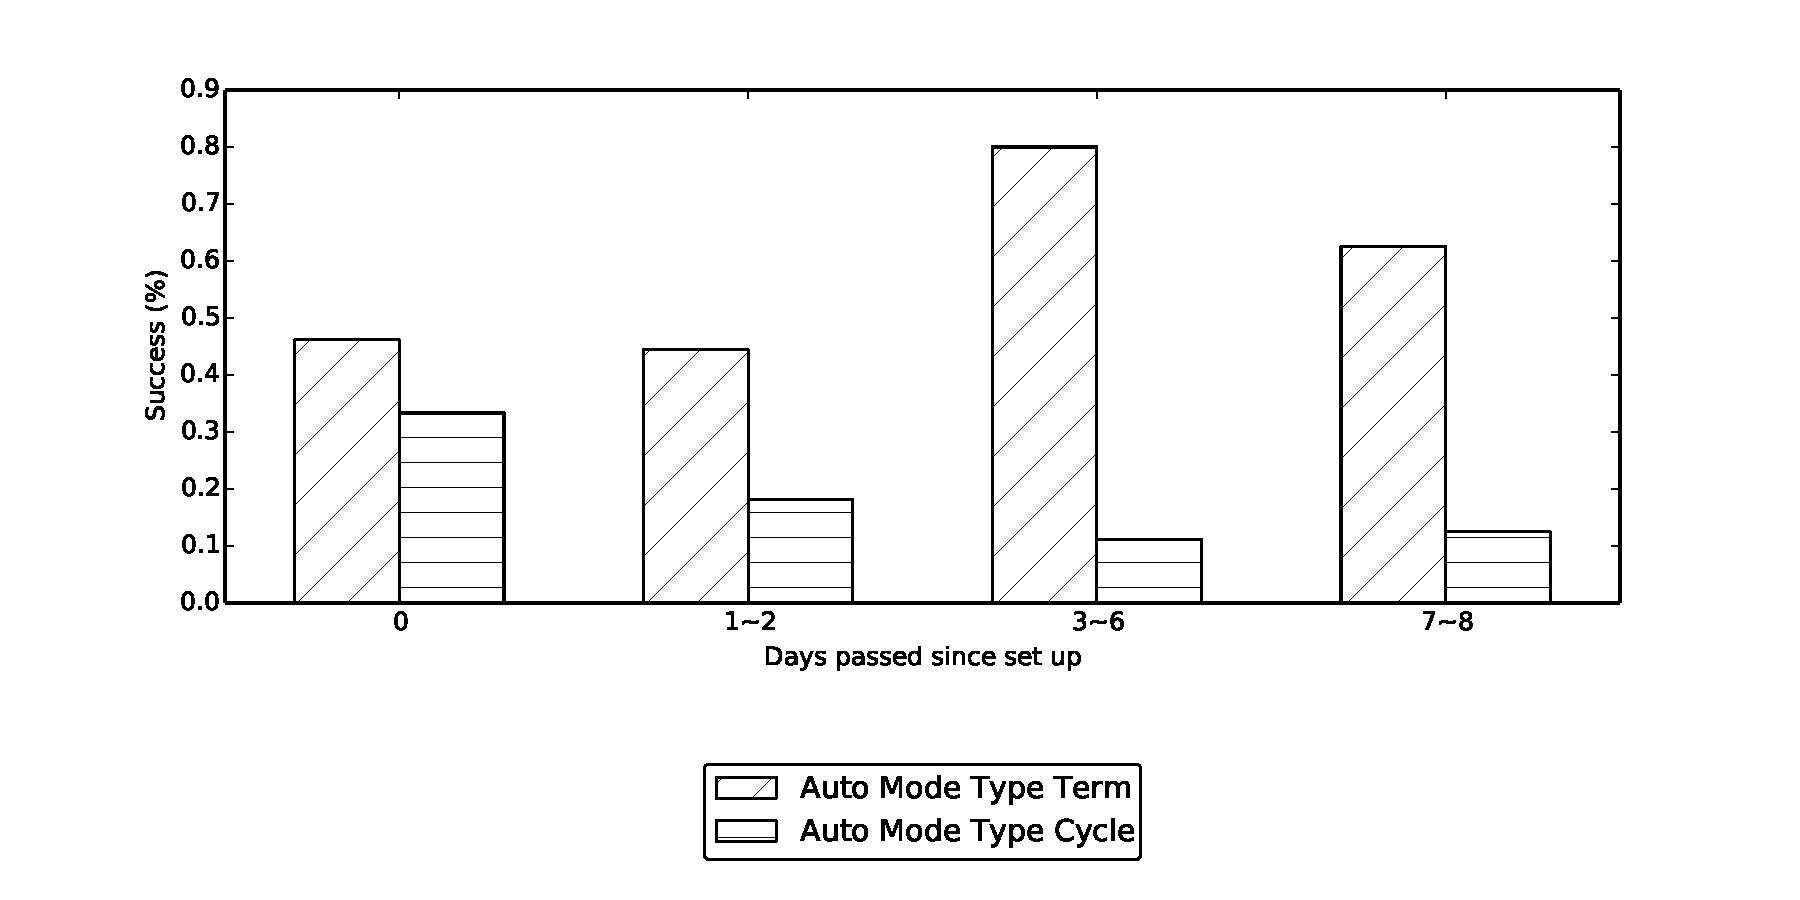
\epsfig{file=resource/ex_auto_term_vs_auto_cycle_rate.pdf,scale=0.5}
%  \end{center}
%  \caption{Auto Mode Type TermとAuto Mode Type Cycleにおける設定時からの経過日数ごとの認証成功率}
%  \label{fig:ex_auto_term_vs_auto_cycle_rate}
%\end{figure}%

%\begin{figure}[ht]
%  \begin{center}
%    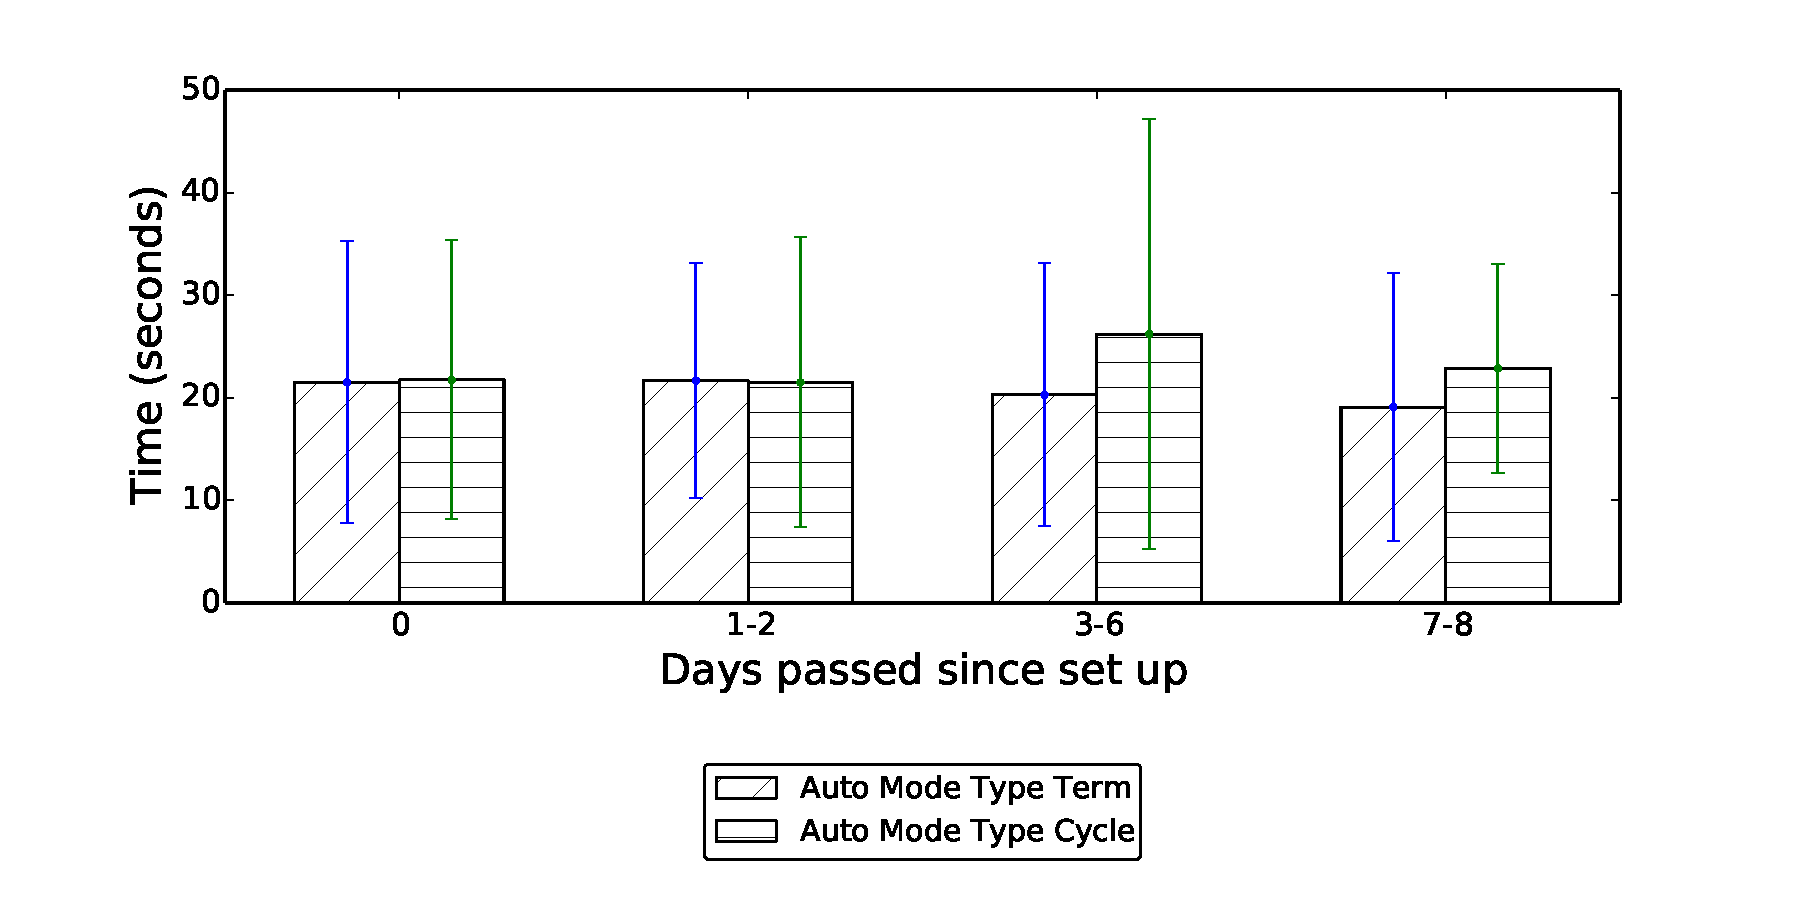
\epsfig{file=resource/ex_auto_term_vs_auto_cycle_time.pdf,scale=0.5}
%  \end{center}
%  \caption{Auto Mode Type TermとAuto Mode Type Cycleにおける設定時からの経過日数ごとの認証時間}
%  \label{fig:ex_auto_term_vs_auto_cycle_time}
%\end{figure}%

%アンケートによる比較結果を図\ref{tab:term_vs_cycle.enquete}に示す.%

%\begin{table}[ht]
%  \begin{center}
%    \small
%    \begin{tabular}{lr}
%      \bhline
%      \multicolumn{2}{l}{どちらのパターンの方が認証操作が楽でしたか?} \\\hline
%      Auto Mode Type Term (\%) & 20 \\
%      Auto Mode Type Cycle (\%) & 5 \\ \hline \hline
%      \multicolumn{2}{l}{どちらのパターンの方が秘密保持しやすかったですか?} \\ \hline
%      Auto Mode Type Term (\%) & 20 \\
%      Auto Mode Type Cycle (\%) & 5 \\ \hline \hline
%      \multicolumn{2}{l}{今後日常的に使わなければならないとすれば,どちらのパターンを使いたいですか?} \\ \hline
%      Auto Mode Type Term (\%) & 20 \\
%      Auto Mode Type Cycle (\%) & 5 \\
%      \bhline
%    \end{tabular}
%  \end{center}
%  \caption{被験者によるAuto Mode Type TermとAuto Mode Type Cycleの比較[NOTICE: 未確定]}
%  \label{tab:term_vs_cycle.enquete}
%\end{table}

%\subsubsection{4つ全ての比較}
%アンケートによる比較結果を図\ref{tab:vs_all.enquete}に示す.
%被験者の○割以上が,△△による設定の方が使いやすさ,覚えやすさ共に優れていると判断した.

%\begin{table}[ht]
%  \begin{center}
%    \small
%    \begin{tabular}{lr}
%      \bhline
%      \multicolumn{2}{l}{どのパターンが最も認証操作が楽でしたか?} \\ \hline
%      Auto Mode Type Term (\%) & 20 \\
%      Auto Mode Type Cycle (\%) & 5 \\
%      Manual Mode (\%) & 30 \\
%      PIN Mode (\%) & 45 \\ \hline \hline
%      \multicolumn{2}{l}{どのパターンが最も秘密保持しやすかったですか?} \\ \hline
%      Auto Mode Type Term (\%) & 20 \\
%      Auto Mode Type Cycle (\%) & 5 \\
%      Manual Mode (\%) & 30 \\
%      PIN Mode (\%) & 45 \\ \hline \hline
%      \multicolumn{2}{l}{今後日常的に使わなければならないとすれば,どのパターンを最も使いたいですか?} \\ \hline
%      Auto Mode Type Term (\%) & 20 \\
%      Auto Mode Type Cycle (\%) & 5 \\
%      Manual Mode (\%) & 30 \\
%      PIN Mode (\%) & 45 \\
%      \bhline
%    \end{tabular}
%  \end{center}
%  \caption{被験者による全パターンにおける比較[NOTICE: 未確定]}
%  \label{tab:vs_all.enquete}
%\end{table}

\newpage

